\chapter{Desarrollo}
\section{Estado del Arte}

Para el desarrollo de este Trabajo de Fin de Grado es necesario utilizar múltiples tecnologías y herramientas. En este capítulo se explicará brevemente el estado actual de los chatbots, las distintas herramientas para desarrollarlos, así como los lenguajes de programación utilizados, qué es el procesamiento natural del lenguaje.

Lo primero que hay que tener en cuenta es que se han desarrollado tres servicios desde cero. Por un lado se ha creado una base de datos no relacional, luego una Api Rest para manejar la base de datos y por último un chatbot que será el que consuma la API y a su vez la base de datos. 


\subsection{Historia de las bases de datos}

Hay que remontarse un poco atrás en el tiempo, concretamente hasta 1880 cuando Herman Hollerith desarrolló una máquina para procesar los datos más rápido de lo que los humanos podían hacerlo. Desarrolló unas tarjetas perforadas mediante las cuales podía realizar un censo de la población completa de Estados Unidos en solo dos años, algo que en esa época era poco más que una quimera. Aun así, la primera vez que se tiene conocimiento del uso del término bases de datos fue en el año 1963 en un simposio celebrado en California y se refiere a ella como un conjunto de información relacionada y que tiene cierta estructura.

Los primeros modelos que fueron desarrollados fueron bases de datos jerárquicas y en red, pero rápidamente se vio que estaban muy limitadas técnicamente y eran demasiado simples. Posteriormente, IBM revolucionó el sector en la década de los 70 creando el modelo relacional de base de datos, mucho más potente y muy bien adoptada por el mundo laboral.
En los 2000 empezaron a aparecer proyectos de código libre que supusieron una competencia en un sector liderado siempre por sistemas privados (IBM y Oracle), entre los más usados destacan MySQL y PostgreSQL. La tendencia a la utilización de sistemas NoSQL contribuyó al detrimento de los sistemas de bases de datos de las grandes empresas. \cite{sanchez2016historia} 

\subsubsection{Bases de Datos Jerárquicas}

Se trata del modelo más antiguo, se ha visto superado por el modelo relacional. El lenguaje de marcado XML utiliza este tipo de modelo para almacenar los datos. El sistema más conocido es el IMS/DB creado por IBM.

\begin{figure}[h]
    \centering
    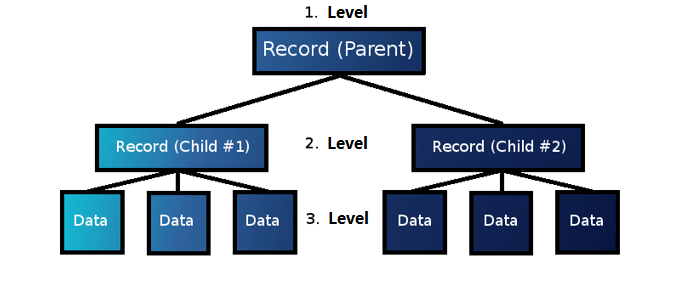
\includegraphics[scale=0.4]{{include/figuras/Jerarquico.png}}
    \caption{Modelo jerárquico}
    \label{fig:bd_jerarquica}
\end{figure}

En este tipo de modelo, cada registro sólo posee un precedente excepto la raíz, formando una estructura arbolada como la que se puede ver en la figura \ref{fig:bd_jerarquica}. En este tipo de modelo, los hijos sólo pueden tener un padre pero un padre puede tener múltiples hijos. Dada esta relación estricta, los niveles que no tengan una relación directa, no pueden interactuar entre ellos y realizar una conexión entre varios árboles tampoco es sencillo. Por este motivo, estas estructuras son consideradas inflexibles aunque por otro lado son muy fáciles de comprender.

\subsubsection{Bases de Datos en Red}

Se desarrolló de manera concurrente al relacional pero con el tiempo se vería superado. No revelan relaciones padre-hijo estrictas sino que cada registro puede tener múltiples precedentes, lo que genera una estructura en red y de ahí su nombre. 
\begin{figure}[h]
    \centering
    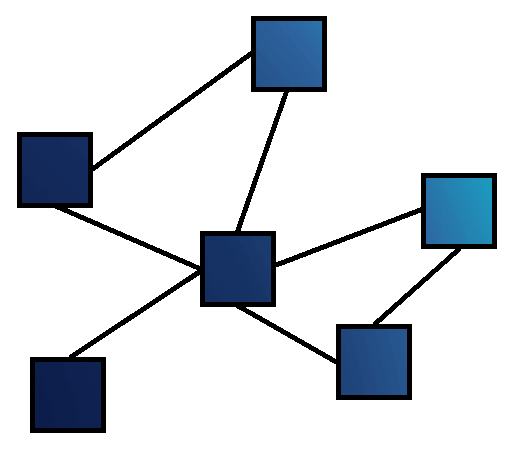
\includegraphics[scale=0.3]{{include/figuras/ModeloEnRed.png}}
    \caption{Modelo de red}
    \label{fig:bd_red}
\end{figure}

Al registro central se tiene acceso desde los otros cinco y desde él, puede accederse a otros cinco registros. En este modelo pueden definirse dependencias, de forma que si accedes al registro superior necesitas pasar por el central para poder alcanzar el registro de la derecha. Hoy en día este modelo de bases de datos se suele utilizar en algunos supercomputadores. Algunos de los modelos más conocidos son el UDS de Siemens y el DMS de Sperry Univac.

\subsubsection{Bases de Datos Relacionales}

Es el modelo más utilizado en la actualidad y es considerado como el estándar de la industria. Normalmente utiliza el lenguaje SQL y se trata de un modelo basado en tablas. Para definir las relaciones se utiliza álgebra relacional y gracias a esta se puede hallar la información de las diferentes relaciones como se puede ver en la figura \ref{fig:bd_relacional}.

\begin{figure}[h]
    \centering
    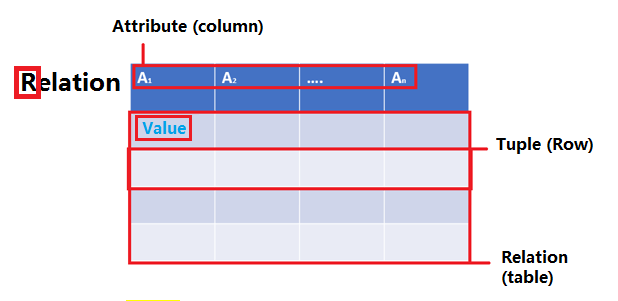
\includegraphics[scale=0.5]{{include/figuras/Relacional.png}}
    \caption{Modelo relacional}
    \label{fig:bd_relacional}
\end{figure}

El modelo relacional funciona mediante tablas independientes que determinan la organización de los datos y sus conexiones. Para poder identificar sin problema un registro es necesario establecer una \textbf{clave primaria}, que habitualmente se trata del primer atributo y no se puede modificar.

\subsubsection{Modelo de Base de Datos Orientado a Objetos}

Surgen a finales de 1980 y a día de hoy han tenido una aplicación muy minoritaria. Este tipo de bases de datos suelen utilizarse en plataformas de lenguajes Java y .NET. La más conocida es \textit{db4o} y destaca por su bajo consumo de memoria. Utilizan un lenguaje OQL, muy parecido a SQL.

\begin{figure}[h]
    \centering
    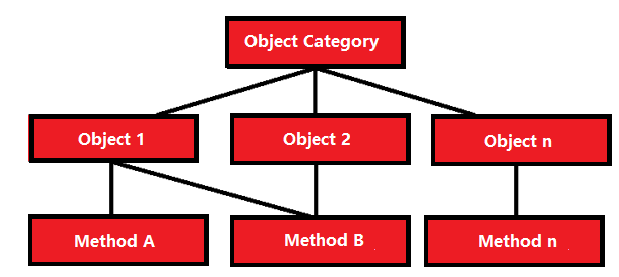
\includegraphics[scale=0.4]{{include/figuras/Objetos.png}}
    \caption{Modelo orientado a objetos}
    \label{fig:bd_objetos}
\end{figure}

En este modelo los datos se almacenan en objetos además de las funciones y los atributos que los definen. Los objetos pueden ser complejos y estar formados por múltiples tipos de datos; se identifican por un identificador de objeto único y se agrupan en clases al igual que en lenguaje de programación orientado a objetos, creando una jerarquía de clases.

\subsubsection{Modelo de Base de Datos Orientado a Documentos}

En este modelo, la unidad mínima de almacenamiento de datos es el documento pero no se deben confundir con los documentos que se generan mediante un procesador de texto. En estos documentos los datos se almacenan como \textbf{pares claves-valor}, como no tienen una definición, los documentos que forman este tipo de bases de datos son muy diferentes entre sí. Cada documento es una unidad cerrada entre sí y establecer relaciones entre documentos no es una tarea sencilla, aunque por otro lado, en este tipo de bases de datos no es necesario establece relaciones.

\begin{figure}[h]
    \centering
    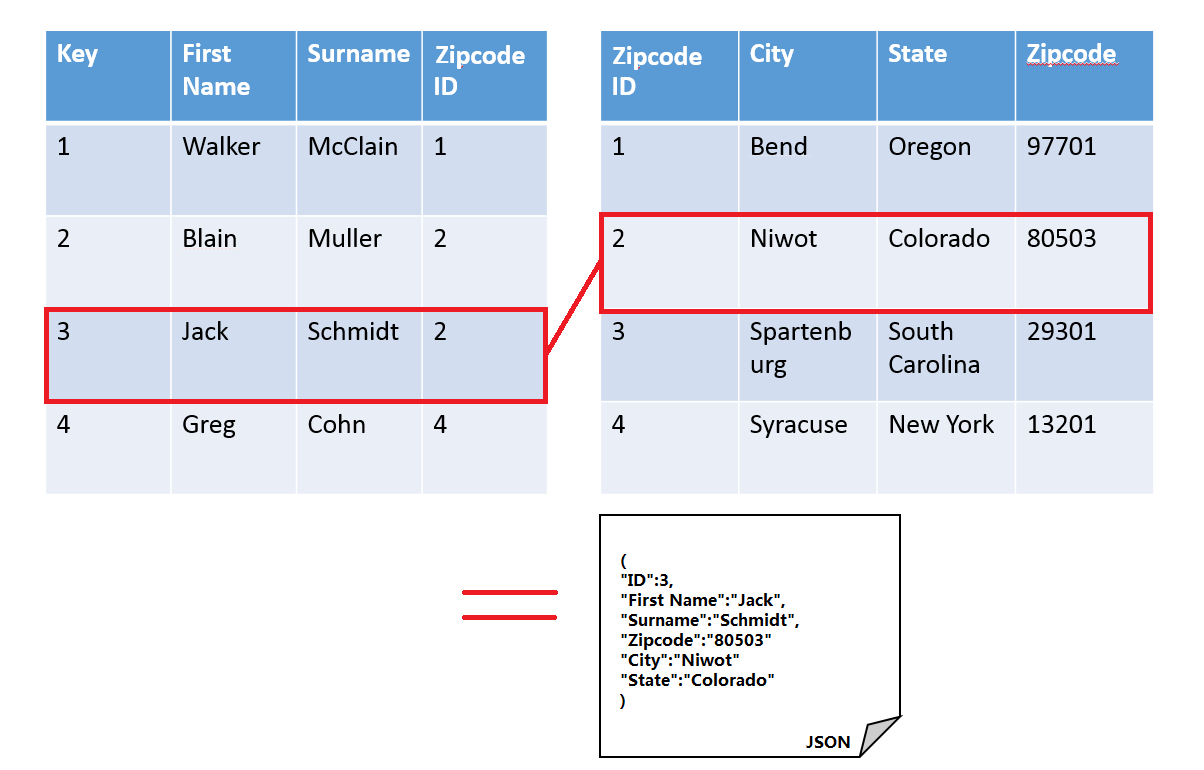
\includegraphics[scale=0.25]{{include/figuras/OrientadaDocumentos.png}}
    \caption{Modelo orientado a documentos}
    \label{fig:bd_documentos}
\end{figure}

La idea fundamental de este tipo de modelos es que los datos que tienen relación se guardan en un mismo documento, esto provoca que el número de consultas a la base de datos sea mucho menor que en una base de datos relacional. Son muy útiles para aplicaciones web debido a que puede almacenarse formularios HTML. Con el avance de la web 2.0 estas bases de datos aumentaron exponencialmente su popularidad y son utilizadas hoy en día por plataformas como Google, Facebook, Twitter, Amazon, etc.
\newpage


\section{Historia de los chatbots}

Un chatbot es una aplicación de software capaz de mantener una conversación con un usuario dando una serie de respuestas automáticas, establecidas con anterioridad a diferentes entradas que pueda dar el usuario. Existen distintas teorías sobre el origen de los chatbots. 

La primera de ellas, defiende que en la década de 1950, el matemático inglés Alan Turing investigó si una máquina sería capaz de imitar las respuestas de un humano mediante el análisis de una conversación de texto entre un humano y una máquina. 

La segunda, más extendida, sitúa el origen en el año 1966 en el Instituto Tecnológico de Massachusetts (MIT), allí el profesor de informática Joseph Weizenbaum desarrolló en el laboratorio de inteligencia artificial el programa \textit{Eliza}, el concepto es que actuara como si se tratase de un terapeuta. Funcionaba de la siguiente manera: examinaba palabras clave que tenía el enunciado del emisor para poder responder con una serie de oraciones que tenía previamente registradas.

En 1972, surgió el chatbot \textit{Parry}, que simulaba ser una persona con esquizofrenia paranoide. A diferencia de Eliza disponía de una estrategia de comunicación cimentada en premisas y ''respuestas emocionales'' en base a las interacciones con los usuarios. \cite{StreamGenerator}

Como detalle curioso, Eliza y Parry fueron puestos a conversar entre sí mediante la red ARPANET \footnote{ARPANET: red de ordenadores creada por el Departamento de Defensa de los Estados Unidos para conectar varias instituciones académicas y estatales.}  

Posteriormente fue desarrollado \textit{Jabberwacky} por el programador inglés Rollo Carpenter, capaz de mantener una conversación mediante la voz. Aunque fue terminado en 1981 no fue hasta 1997 cuando fue publicado online.

A partir del año 2006 han surgido una gran cantidad de chatbots entre los que cabe destacar:

IBM Watson, nombrado así por el primer director ejecutivo de IBM. En un principio fue desarrollado para responder preguntas y respuestas ideadas por humanos para el concurso Jeopardy. El concurso es el típico de preguntas y respuestas solo que las preguntas son formuladas mediante juegos de palabras y giros lingüisticos. Se presentó al concurso en 2011 por primera vez y fue capaz de ganar a dos especialistas. A partir de ese instante, ha pasado por varias adaptaciones utilizando procesamiento de lenguaje natural y machine learning\footnote{Machine Learning: disciplina dentro de la Inteligencia Artificial que crea sistemas y software capaces de aprender automáticamente} para procesar una gran cantidad de datos. En 2013, IBM anunció que Watson podía ser utilizado para la toma de decisiones en el tratamiento del cáncer de pulmón. 

Tal vez el chatbot más conocido mundialmente sea el asistente virtual desarrollado por Apple, \textit{Siri}. Utiliza consultas dadas mediante comandos de voz para ayudar al usuario de diversas formas, realizar tareas, recordatorios, búsquedas y modificar configuraciones del sistema.

De este mismo estilo tenemos los chatbot \textit{Alexa} creado por Amazon,\textit{Cortana} desarrollado por Microsoft y \textit{Google Now} desarrollado por Google


\section{Frameworks y librerías para el desarrollo de chatbots}

Lo primero qué debemos conocer es la diferencia entre un \textit{Framework} y una librería. Un framework es un tipo de estructura con una serie de archivos y pautas que se utiliza para desarrollar proyectos con una estructura y metodología, es decir, algo así como una plantilla que simplifica la creación de una solución. 
Por otro lado, una librería es uno o varios archivos escritos en algún tipo de lenguaje de programación, que proporcionan varias funcionalidades. Al contrario que un framework, una librería no establece la estructura sobre cómo debe realizarse el desarrollo, sino que da funcionalidades genéricas que han sido programadas con anterioridad y evitan que haya que escribir código de más, aumentando la calidad del código y reduciendo el tiempo de desarrollo.

\section{Frameworks}

\subsubsection{DialogFlow}

Framework de desarrollo de chatbots creado en 2010 y mantenido por Google\cite{Dialogflow}. Es capaz de comprender el lenguaje natural y nos brinda herramientas para la fabricación de diálogos y la recreación de conversaciones. Destaca por la gran cantidad de interfaces de conversación en los que se puede desplegar (Google home, google assistant, wereables, teléfonos, coches). Tiene soporte para más de 14 idiomas y es capaz de resolver abreviaturas y funcionar con faltas de ortografía. 
Posee una interfaz muy intuitiva y permite crear chatbots en una cantidad pequeña de tiempo. 
\begin{figure}[ht]
    \centering
    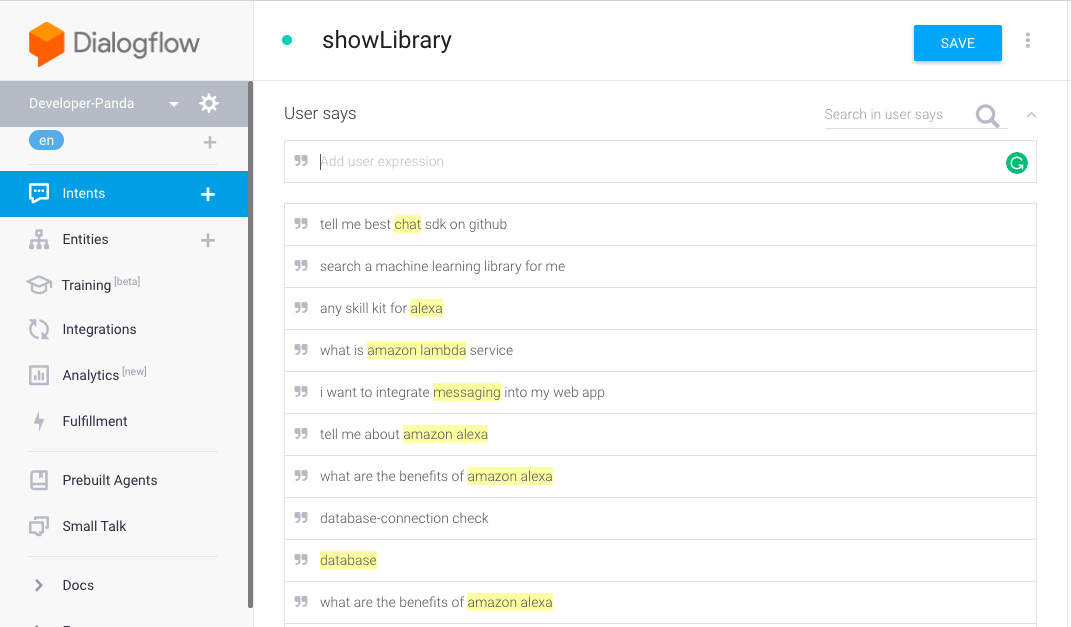
\includegraphics[scale=0.4]{{include/figuras/DialogFlow.png}}
    \caption{Interfaz de dialogflow}
    \label{fig:dialogflow_gui}
\end{figure}


\subsubsection{Microsoft Bot Framework}
Desarrollado por Microsoft, crea chatbots rapidamente a través de la herramienta Microsoft Bot Builder y los conecta con Azure Bot Service, lo que nos permite una rápida creación del bot ya que nos proporciona diversas plantillas para seleccionar cuando se está creando el bot y nos brinda todas las mejoras de la nube creada por Microsoft. Puede editarse con directamente desde la página web usando el editor de Azure o algún IDE de desarrollo como Visual Studio o Visual Studio Code \cite{MicrosoftBotBuilder}. Posee su propio sistema de procesamiento natural del lenguaje llamado LUIS (\textit{Language Understanding Intelligent Service}).   

\subsubsection{IBM Watson}
Creado por IBM, es capaz de comprender y responder a las preguntas de los usuarios mediante lenguaje natural \cite{MicrosoftBotBuilder}. Watson está compuesto actualmente por un clúster de al menos 750 servidores \textit{IBM Power 750}, con unos 16 TB de memoria RAM, lo que proporciona una potencia de cálculo bruto de unos \textbf{80 petaflops}, convirtiéndolo así en uno de los supercomputadores más potentes del mundo. 

\subsubsection{Amazon Lex}
Creado y gestionado por Amazon, permite establecer comuncicaciones con todos sus productos Eco y con su asistente virtual Alexa. Es una de las mejores herramientas en cuanto a conversión de voz a texto. Con esta herramienta se pueden crear bots con un lenguaje natural sofisticado. A diferencia de los anteriores, tiene una interfaz más intuitiva para principiantes aunque por el contrario, dispone de menos herramientas, aunque posee todas las necesarias en un chatbot.

\subsubsection{Rasa}
Por último cabe destacar Rasa, una framework \textit{Open Source} de machine learning que nos permite crear conexiones entre las máquinas y el usuario. Posee herramientas para entender al usuario mediante el componente Rasa NLU (Natural Langugage Understanding), generar el diálogo con Rasa NLG (Natural Language Generation) y un motor (Rasa Core) capaz de definir cuál será la siguiente acción a tomar en función del mensaje transmitido por el usuario.   


\section{Librerías}
Vamos a analizar las librerías existentes para el lenguaje de programación Python, debido a que se trata de un lenguaje simple, elegante ordenado y portable.

\subsubsection{Chatterbot}
Se trata de una librería de machine learning basada en las conversaciones y diálogos tradicionales. Lo más destacable de esta librería es que está diseñada de tal manera que permite crear chatbots que soporten varios idiomas. 

Es también compatible con librerías para aportar más funcionalidades como puede ser la conversión de texto a voz y así poder interactuar con el usuario sin necesidad de escribir.

\subsubsection{Natural Language ToolKit} NTLK por sus siglas en inglés, se trata de una plataforma para crear chatbots con lenguaje humano. Dispone de funcionalidades muy interesantes desde el punto de vista del reconocimiento del lenguage como la tokenización , derivación, etiquetado, análisis y razonamiento semántico.

\subsubsection{ChatbotAI} Nos permite crear un chatbot con muy pocas líneas de código. Genera un controlador del chat y bots con inteligencia artificial que permiten una integración muy sencilla con API Rest. Esta inteligencia artificial nos genera múltiples características como aprender, memorizar, manejar conversaciones según el tema \cite{chatbotAI}. 

\subsubsection{Tensorflow} Es uan plataforma de código abierto gestionada por Google. Se trata de una biblioteca de aprendizaje automático con la que es posible construir y entrenar redes neuronales para detectar patrones y correlaciones en el aprendizaje y razonamiento de los humanos. 

\section{Arquitectura del Trabajo}

Este Trabajo de Fin de Grado está incluido dentro de una estructura que está formada por varios proyectos que se explicarán a continuación.
En el ordenador instalado en la estación de Fuenlabrada está colocado el programa \textit{Echoes Watcher} \cite{echoesWatcher}. Este programa lee el archivo de configuración  generado por Echoes para obtener datos de interés (peak, directorio, nombre estación, etc) y según se van generando ficheros de detecciones, el programa mediante un programa de monitorización, lee esos ficheros y en caso de encontrar alguna detección, se envían los datos a través de un Broker MQTT \cite{singh2015secure} al equipo ubicado en el Centro de Supercomputación y Visualización de Madrid (Cesvima).

Todos los días se procede a hacer un backup de los datos sin filtrar a otro computador del proyecto ubicado en la Escuela Técnica Superior de Ingeniería y Diseño Industrial (ESTIDI).

En el Cesvima se encuentra ubicado el programa StreamGenerator \cite{StreamGenerator}. Este programa está suscrito al broker y puede recibir datos de configuración de la estación y datos de las detecciones. Cuando recibe datos de configuración de las detecciones genera un fichero de liquidsoap \cite{liquidsoap} si no existe o si ha cambiado la configuración de la estación. Este fichero liquidsoap genera una lista de reproducción que está ubicada en el Instituto Astrofísico de Canarias y se trata de un bucle infinito de ruido (basado en el archivo de configuración) y a medida que le llegan detecciones de una estación se altera dicha lista de reproducción para añadir los sonidos generados con la detección que recibe del broker, y una vez que el sonido es reproducido, se borra. 
Por cada estación existente hay una lista de reproducción, lo que significa que existe un proceso liquidsoap ejecutándose por cada estación.  


//TODO









A continuación, se mostrará la arquitectura general del sistema desarrollado.

\begin{figure}[h]
    \centering
    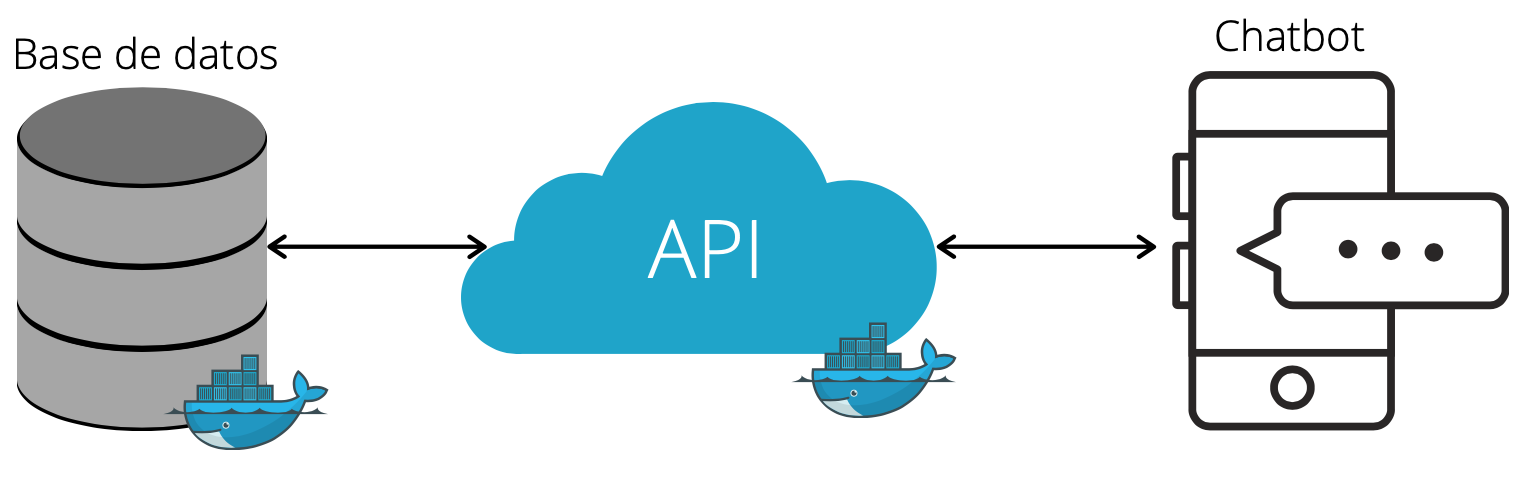
\includegraphics[scale=0.4]{{include/figuras/ArquitecturaGeneral.png}}
    \caption{Arquitectura general}
    \label{fig:arquitectura_general}
\end{figure}

Como se puede observar en la figura \ref{fig:arquitectura_general}, la API RestFul es el software encargado de gestionar e interactuar con la base de datos, sirviendo los datos a los usuarios. Para que el proyecto sea lo más escalable posible se ha decidido separar los servicios de forma que estén débilmente acopladas. 

\subsection{Base de Datos}
Para el proyecto Sonidos del Cielo hemos elegido MongoDB. En gran parte debido a que es una herramienta perfecta para entornos con bajos recursos de computación, no es necesario pagar ningún tipo de licencia, posee una gran comunidad y muy buena documentación, además de muy escalable. La ventaja principal de MongoDB es que los documentos no tienen que seguir una estructura definida, es decir, se puede trabajar con documentos independientes, modificar el contenido de uno de forma individual y no afectar a la estructura.

\begin{figure}[h]
    \centering
    
\includegraphics[scale=0.2]{include/figuras/mongo.png}
    \caption{Logo de MongoDB}
    \label{fig:mongo}
\end{figure}

La característica principal de MongoDB es la velocidad, dado que está escrito en C++ tiene la capacidad de aprovechar los recursos del sistema de una manera eficiente, es decir, tiene un gran balance entre funcionalidad y rendimiento gracias a su sistema de consulta de contenidos. Las características principales de la plataforma son:

\begin{itemize}
    \item Consultas ad-hoc: se pueden realizar todo tipo de consultas. Podemos buscar por campos como si de una base de datos relacional se tratase pero además podemos buscar por rango, mediante expresiones regulares.
    \item Indexación: el concepto es muy parecido al utilizado en las bases de datos relacionales, sin embargo, en MongoDB se puede indexar cualquier campo documentado e incluir múltiples índices secundarios.
    \item Balanceo de carga: MongoDB posee la capacidad de ejecutarse de manera simultánea en múltiples servidores, dando un servicio de balanceo de carga o de replicación de datos, de manera que es posible mantener el funcionamiento del sistema en caso de un fallo de hardware.
    \item Almacenamiento de archivos: puede ser utilizado también como almacenamiento de archivos, esta función, conocida como GridFS está incluida en la distribución oficial y permite manipular archivos y su contenido.
    \item Ejecución de JavaScript en el lado del servidor: es posible realizar consultas utilizando código escrito en JavaScript, haciendo que estas sean enviadas directamente a la base de datos para ser ejecutadas.
\end{itemize}

\subsubsection{Funcionamiento de MongoDB}
MongoDB está orientado a documentos. Esto significa que en lugar de guardar los datos en registros se guardan en documentos BSON, que no es otra cosa que un fichero JSON binario.
Esto es una de las grandes diferencias respecto a las bases de datos relacionales. 
MongoDb se compone de colecciones que a su vez está formado por documentos documentos. 

Si hiciésemos una comparación con los elementos de una base de datos relacional, se trataría de una tabla. Dentro de cada colección existen múltiples documentos que están compuestos de pares Clave-Valor. 
La principal diferencia respecto a una base de datos relacional es que no es necesario que los documentos de una misma colección tengan el mismo formato ni los mismos campos.
\newpage
\subsubsection{Diseño de la Base de Datos}

Las tablas obtenemos desde ficheros que se encuentran en un servidor del Spanish Virual Observatory (SVO) dentro del Departamento de Arquitectura y Tecnología de Sistemas Informáticos (DATSI) de la Escuela Técnica Superior de Ingenieros Informáticos de la Universidad Politécnica de Madrid. A partir de este fichero se crean las tablas que se aprecian en la figura \ref{fig:tablas_base_datos}

\begin{figure}[h]
    \centering
    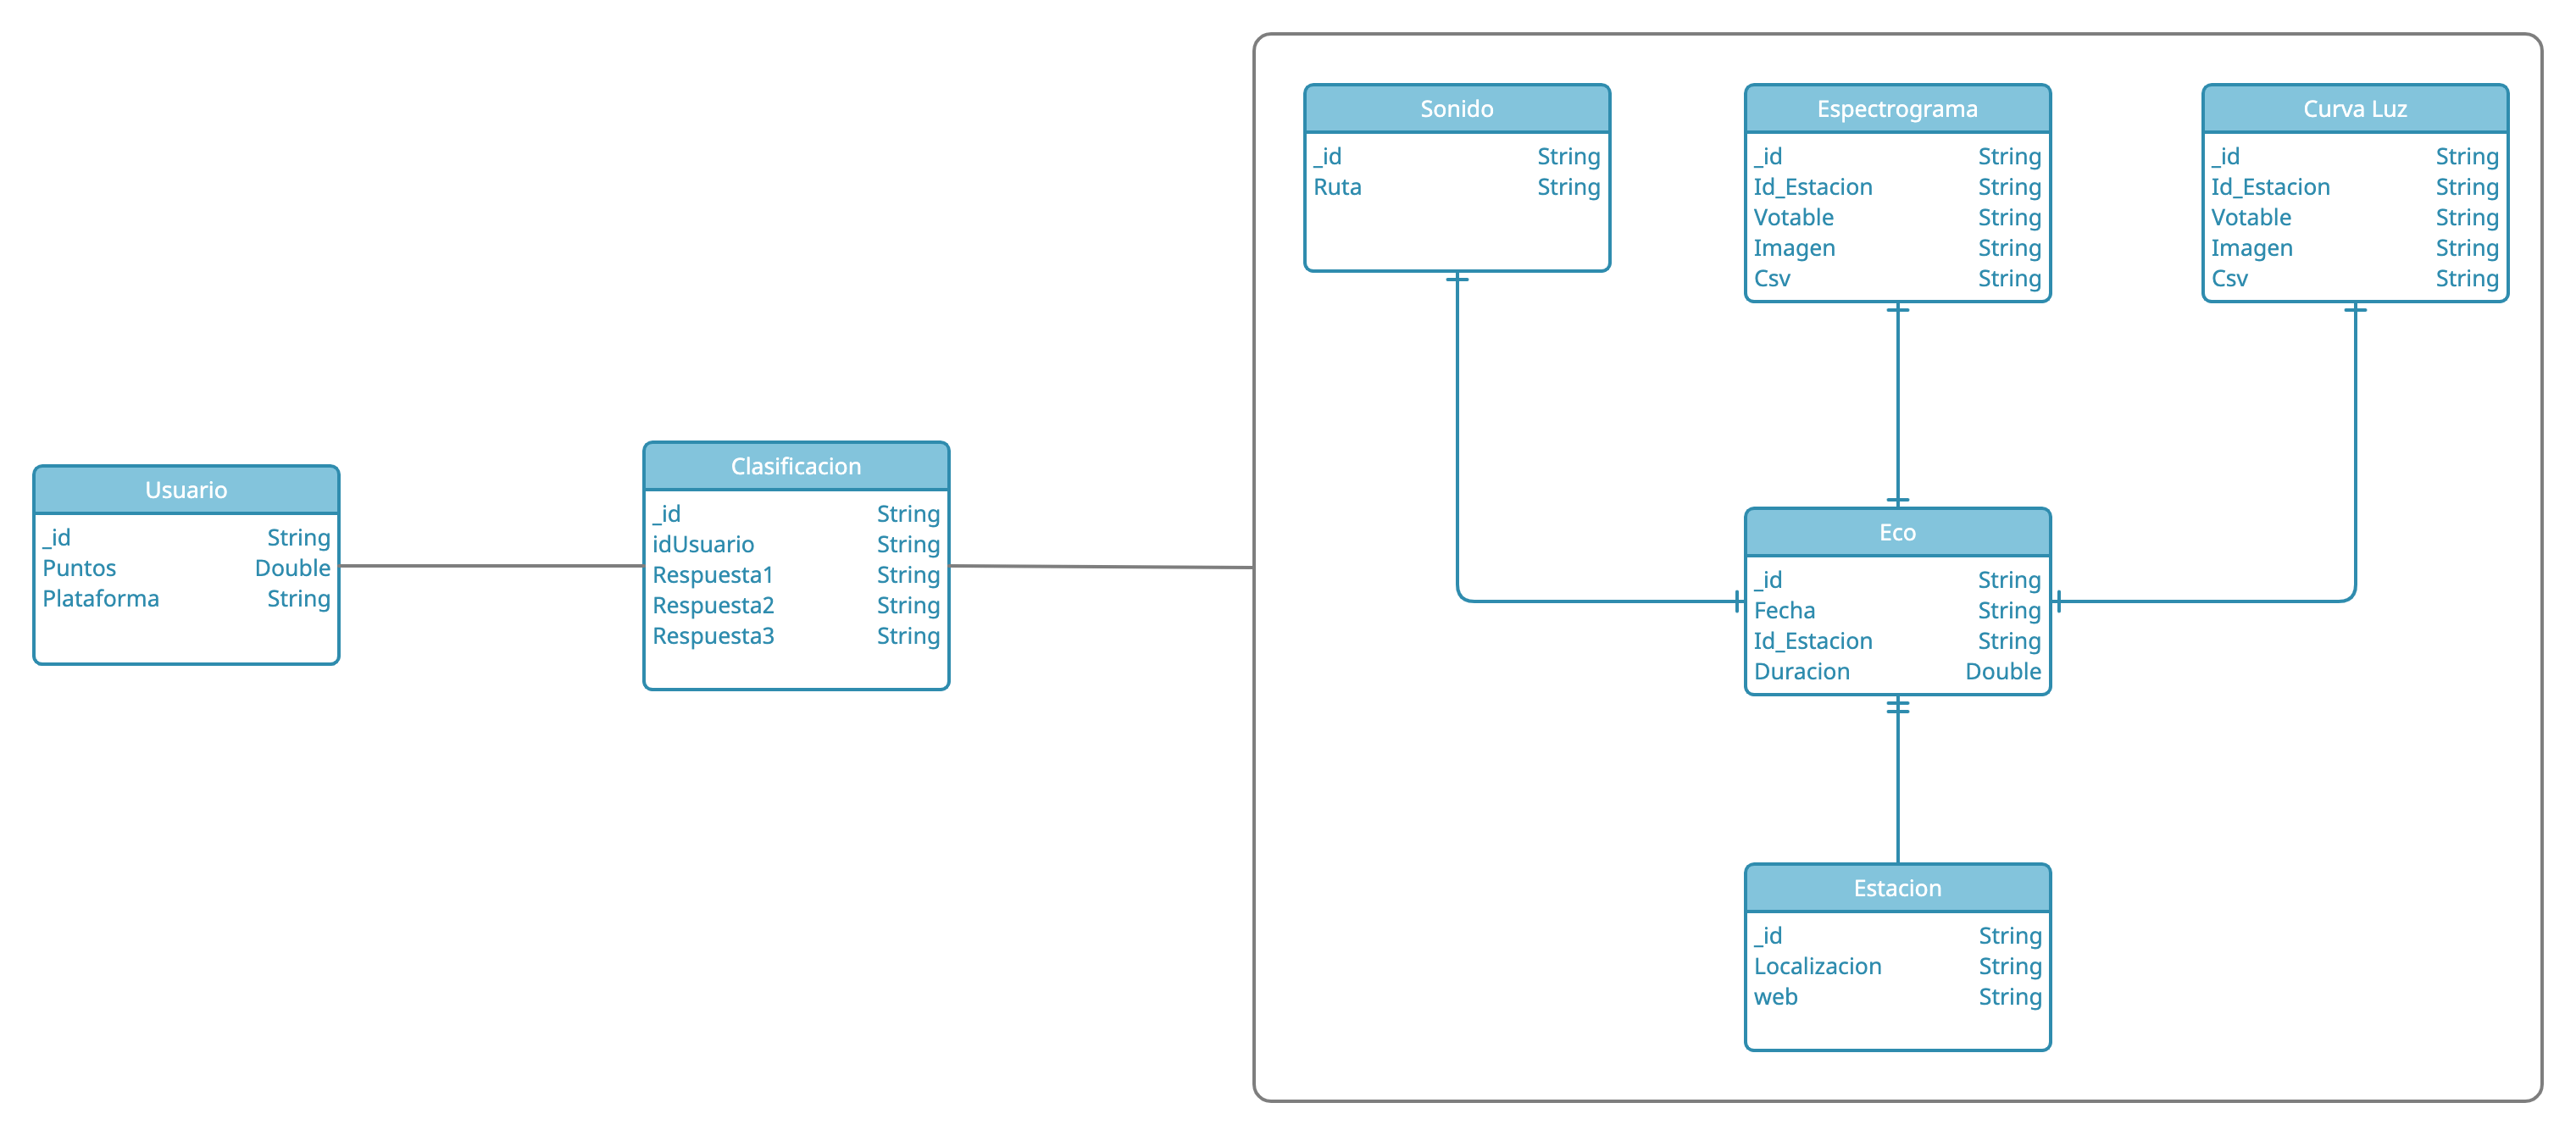
\includegraphics[scale=0.6]{include/figuras/Tablas.png}
    \caption{Colecciones de la base de datos}
    \label{fig:tablas_base_datos}
\end{figure}

Aunque hemos explicado anteriormente que no es estrictamente necesario que existan relaciones entre las tablas, en este proyecto si que es necesario puesto que varias tablas proceden del mismo meteoroide.



\subsection{Arquitectura aplicación RestFul}

La aplicación RestFul no es más que el software que hace de intermediario para enviar información de la base de datos al cliente o para insertar datos desde el cliente a la base de datos. El cliente es aquel que consume la información, en nuestro caso, el chatbot. El servidor se ha desarrollado en Node.js. Fue diseñado para la construcción de aplicaciones escalables, siendo un punto muy a favor para nuestra elección. 

Además, puesto que queremos tratar las peticiones de los usuarios, la mejor manera de hacerlo es de forma asíncrona así no es necesario esperar a que se traten las peticiones realizadas con anterioridad.


\begin{figure}[h]
    \centering
    
\includegraphics[scale=0.2]{include/figuras/node.jpg}
    \caption{Logo de Node.js}
    \label{fig:node}
\end{figure}

Node.js es un entorno de ejecución de JavaScript \cite{javascript} orientado a eventos asíncronos


\subsection{}

\subsection{Sección 1 de apartado 1 de capítulo 2}

\subsubsection{Sub sección 1}

\subsubsection{Sub sección 2}

\subsection{Sección 2 de apartado 1 de capítulo 2}

\section{Apartado 2 de capítulo 2}

\section{Apartado 3 de capítulo 2}
